\documentclass[captions=tableheading]{scrartcl}
\usepackage[aux]{rerunfilecheck}

\usepackage{fontspec}
\usepackage[main=ngerman]{babel}
\usepackage[unicode]{hyperref}
\usepackage{bookmark}
\usepackage{booktabs}
\usepackage{amsmath}
\usepackage{amssymb}
\usepackage{mathtools}
\usepackage{graphicx}
\usepackage{grffile}
\usepackage{scrhack}
\usepackage{float}
\usepackage{pdfpages}
\floatplacement{figure}{htbp}
\setmainfont{Libertinus Serif}
\subject{Versuchsnummer: 303}
\title{Der Lock-In-Verstärker}
\author{Richard Leven \\ \href{mailto:richard.leven@tu-dortmund.de}{richard.leven@tu-dortmund.de}
 \and Joell - D. Jones \\ \href{mailto:joell-david.jones@tu-dortmund.de}{joell-david.jones@tu-dortmund.de}} 
\date{
    Durchführung: 19.11.2019\\
    Abgabe: 26.11.2019
}
\publishers{TU Dortmund - Fachschaft Physik}
\begin{document}
\maketitle
\newpage
\section{Ziel}
Die Intention in diesem Versuch ist es den Lock-In-Schalter kennenzulernen, da das Unterdrücken von Rauschsignalen im Alltag, doch vor allem in der Wissenschaft wichtig ist. In der Wissenschaft will man in der Praxis nämlich Ungenauigkeiten und "Schmutzfaktoren" so gut wie möglich beseitigen, sodass die Diskrepanzen der Messwerte in Schach gehalten werden können. 
\section{Theorie}
Ein Lock-In-Verstärker liefert eine klare Gleichspannung bei einem Input von einem Signal mit Rauschen und einem Referenzsignal.
Zuerst werden die zu hohen und zu niedrigen Frequenzen des rauschenden Nutzsignals mit einem Bandpassfilter eliminiert.
Ein Referenzsignal mit gleicher Phase und Frequenz wird nun mit dem Nutzsignal vermischt, also miteinander mit der Frequenz \(\omega_0\) multipliziert. Das resultierende Signal wird mit einem Tiefpassfilter integriert und über mehrere Perioden gemittelt, sodass eine Gleichspannung erzeugt wird, die rauschfrei ist, da die synchronisierten Rauschteile des vermischten Signals herausgemittelt werden.
\section{Versuchsdurchführung}
\begin{figure}
\centering
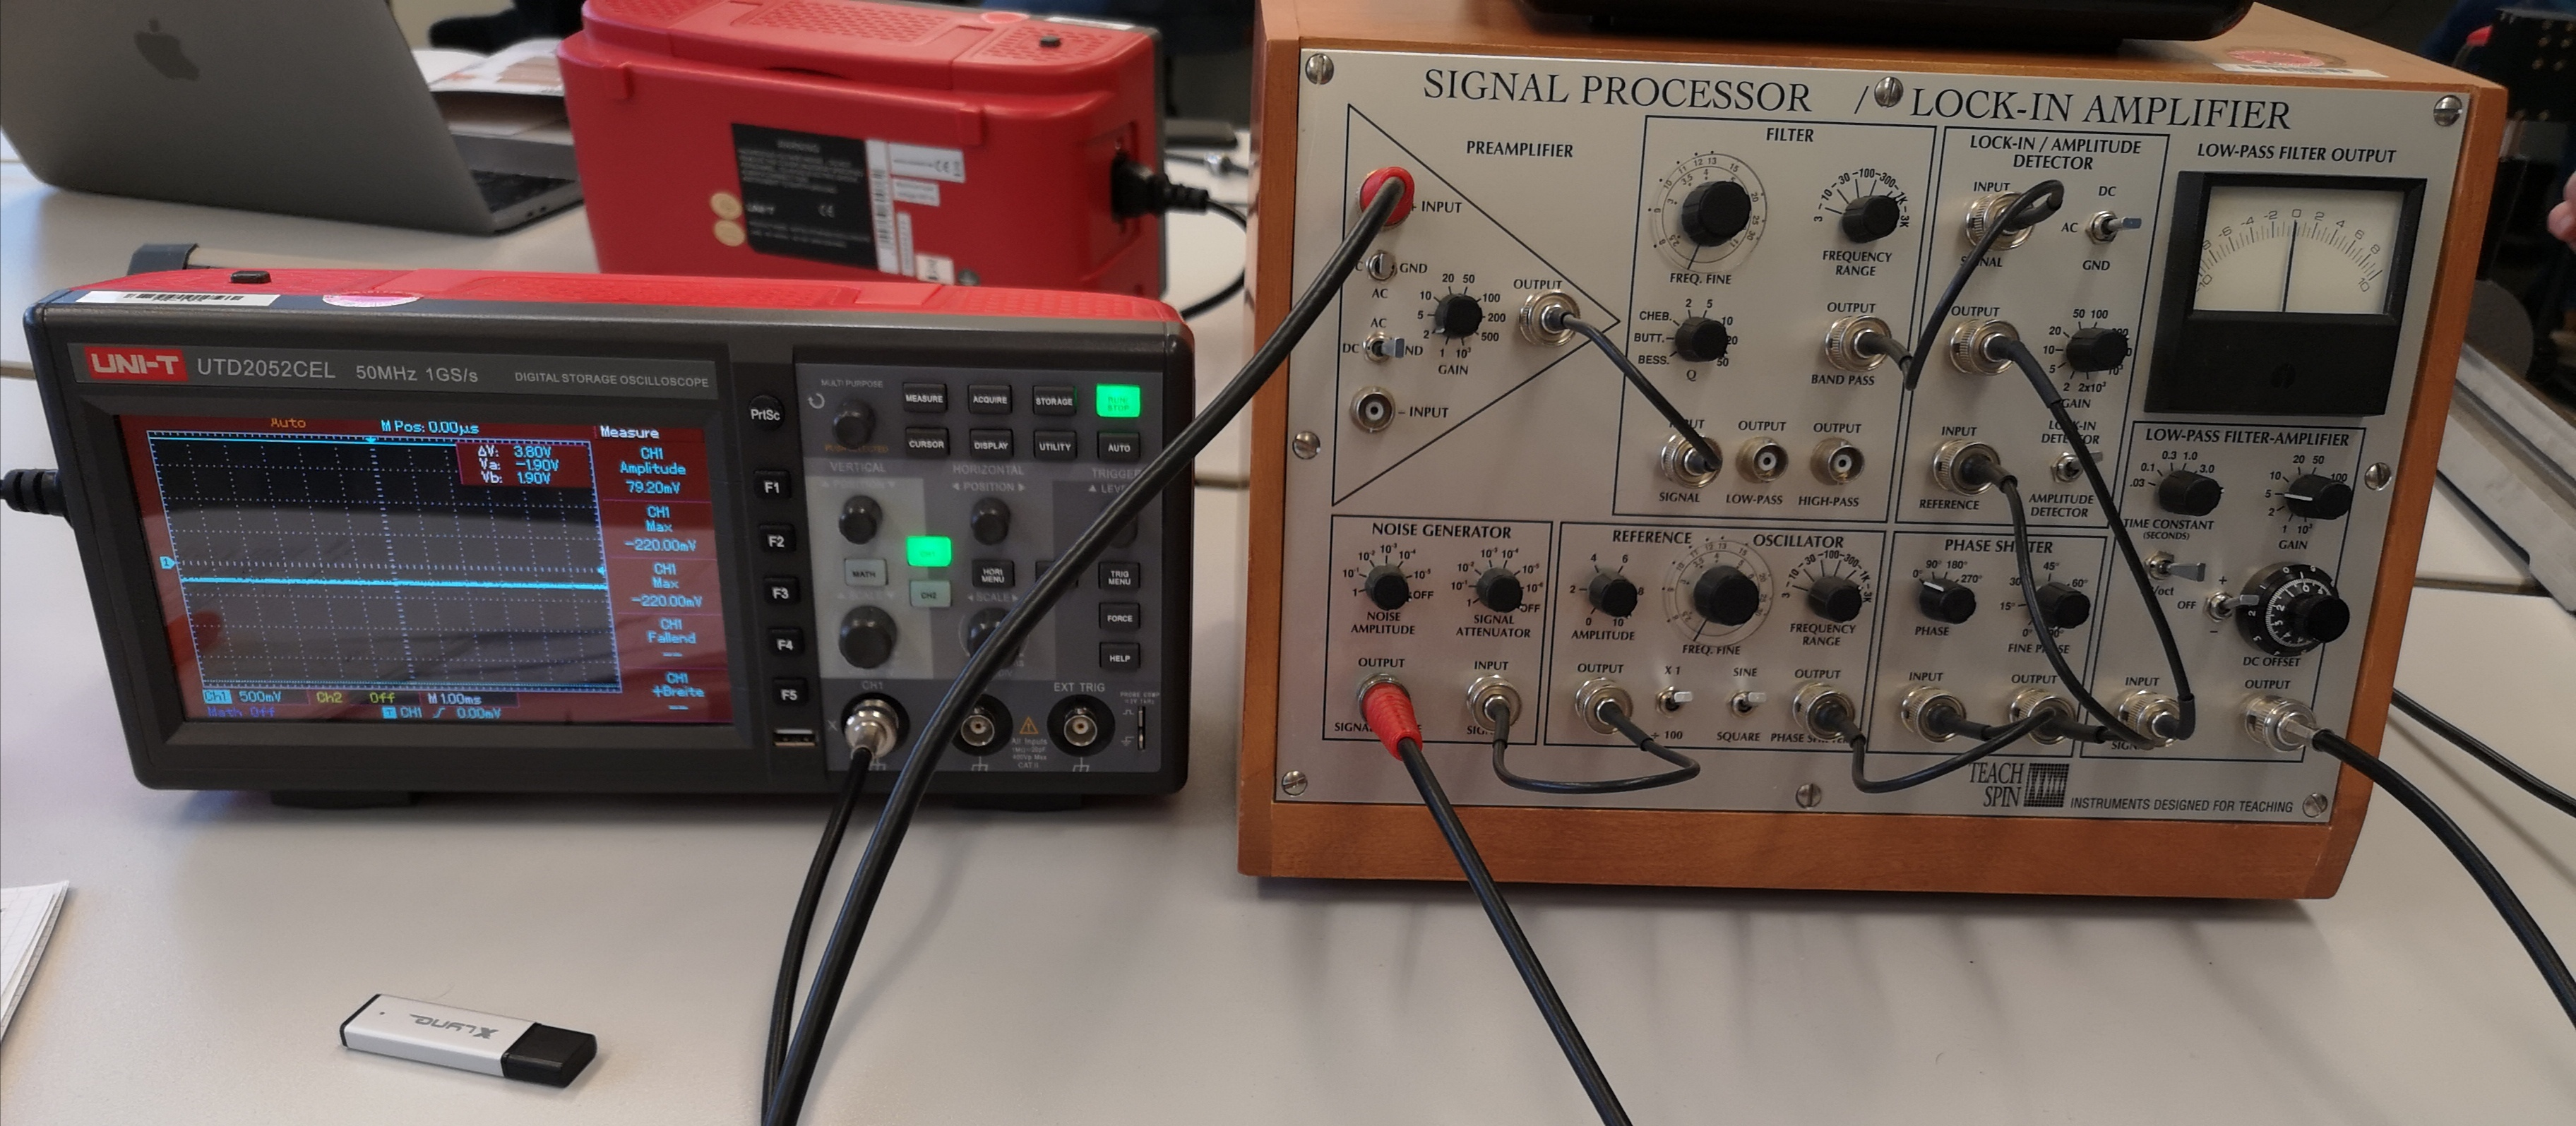
\includegraphics[scale=0.07]{Lock_In Bilder/Versauf.jpg}
\caption{Der Versuchsaufbau}
\label{fig:versau}
\end{figure}

Um den Schaltkreis des Lock-In-Verstärkers zunächst einmal näher kennenzulernen, wurden die Outputs am Lock-In-Verstärker variiert, sodass einmal der Tiefpass überbrückt wurde und einmal nicht.
\\
Die Outputs wurden an das Oszilloskop angeschlossen und an den Bildschirm angepasst, um ein klares Bild zu bekommen. So konnten die konstanten und variablen Spannungs-Outputs ermittelt werden.  
\\ 
Ohne den Noise-Generator wurde nun ein sinusförmiges Eingangssignal mit einer Frequenz von 1000 Hz und einer Spannung von 0,01 V ausgegeben und mit einem weiteren Sinussignal identischer Frequenz vermischt. Daraufhin wurde der Tiefpass erneut überbrückt und fünf verschiedene Phaseneinstellungen eingestellt: \(0°, 45°, 90°, 135°, 180°\).
\\ 
Dasselbe Prozedere folgt hinterher mit Noise-Generator; das Rauschen wurde auf $10^{-3}$ eingestellt, was der Größenordnung der Spannung des Signals entsprach.
\\ 
Ganz zum Schluss wurde der Schaltkreis leicht modifiziert, sodass nun der Output vom Lock-In-Verstärker nicht mehr nach dem Tiefpass erfolgte, sondern bereits nach dem Lock-In. 
Gleichzeitig wurde auch ein Signal zum Tiefpass-Input gelegt, sodass der Versuchsaufbau nun wie die Schaltkreis-Skizze in der Abbildung 5 geschaltet war. Die LED wurde mit einer Frequenz von 300 Hz betrieben. 
\\
Für eine genauere Messung wurde der Raum zusätzlich verdunkelt und teilweise wurde das Experiment mit Objekten wie Taschen und Jacken zugedeckt. Das Ziel des Ganzen war es ein maximaler Abstand \(r_{max}\), in der die Photodiode das Licht einer LED noch messen kann nachzuweisen.
\newpage
\section{Auswertung}
    \begin{itemize}
        \item{Kennenlernen des Lock-In-Verstärkers \\}
            \begin{figure}
                \centering
                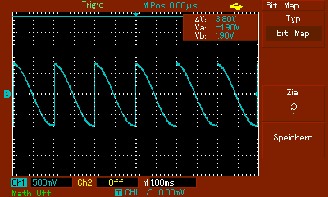
\includegraphics{Lock_In Bilder/Aufgabe 1/MAP001.pdf}
                \caption{Die Sägezahnschwingung}
                \label{fig:sawsig}
            \end{figure}
            \\
            In Abbildung \ref{fig:sawsig} wurde der Output nach dem Lock-In abgegriffen und nicht nach dem Tiefpass.
            Eine Sägezahnschwingung ist das Resultat. 
            \\
            \begin{figure}
                \centering
                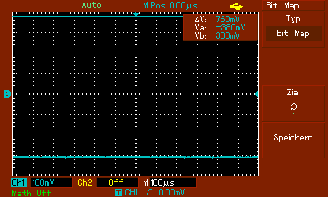
\includegraphics{Lock_In Bilder/Aufgabe 1/MAP002.pdf}
                \caption{Die Gleichspannung}
                \label{fig:flatsig}
            \end{figure}
            \\
            In Abbildung \ref{fig:flatsig} wurde der Output nach dem Tiefpass abgegriffen.
            Eine Gleichspannung im negativen Bereich ist das Resultat.
            Sie entsteht, wenn die Sägezahnschwingung aus Abbildung \ref{fig:sawsig} durch den Tiefpass verändert wird.
        \newpage
        \item{Eingangssignal ohne Noise-Generator \\}
            
            \begin{figure}
                \centering
                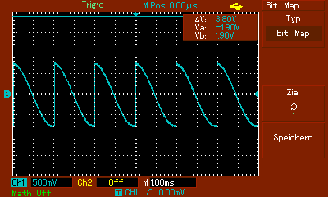
\includegraphics{Lock_In Bilder/Aufgabe 2/MAP001.pdf}
                \caption{AC-Signal bei 0° Phase}
                \label{fig:0sig}
            \end{figure}
            \\
           
            \begin{figure}
                \centering
                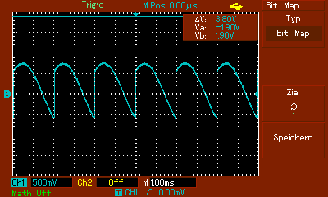
\includegraphics{Lock_In Bilder/Aufgabe 2/MAP002.pdf}
                \caption{AC-Signal bei 45° Phase}
                \label{fig:45sig}
            \end{figure}
            \\
           
            \begin{figure}
                \centering
                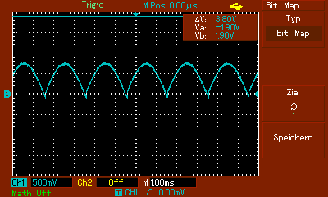
\includegraphics{Lock_In Bilder/Aufgabe 2/MAP003.pdf}
                \caption{AC-Signal bei 90° Phase}
                \label{fig:90sig}
            \end{figure}
            \\
            \newpage
         
            \begin{figure}
                \centering
                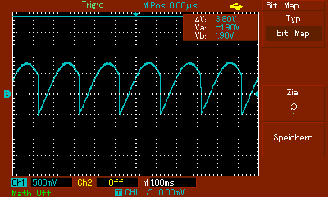
\includegraphics{Lock_In Bilder/Aufgabe 2/MAP004.pdf}
                \caption{AC-Signal bei 135° Phase}
                \label{fig:135sig}
            \end{figure}
            \\
            
            \begin{figure}
                \centering
                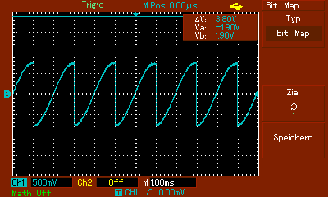
\includegraphics{Lock_In Bilder/Aufgabe 2/MAP005.pdf}
                \caption{AC-Signal bei 180° Phase}
                \label{fig:180sig}
            \end{figure}
            \\
            Die Signale entsprechen der theoretischen Vorstellung, wenn \(U_{ref}\) um die jeweiligen Grade verschoben wird.
    
        \newpage
        \item{Eingangssignal mit Noise-Generator \\}
          
            \begin{figure}
                \centering
                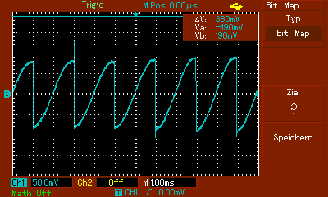
\includegraphics{Lock_In Bilder/Aufgabe 3/MAP001.pdf}
                \caption{AC-Signal bei 0° Phase}
                \label{fig:0sig2}
            \end{figure}
            \\
           
            \begin{figure}
                \centering
                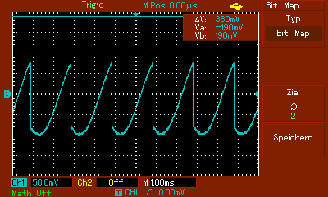
\includegraphics{Lock_In Bilder/Aufgabe 3/MAP002.pdf}
                \caption{AC-Signal bei 45° Phase}
                \label{fig:45sig2}
            \end{figure}
            \\
           
            \begin{figure}
                \centering
                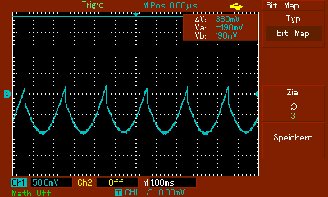
\includegraphics{Lock_In Bilder/Aufgabe 3/MAP003.pdf}
                \caption{AC-Signal bei 90° Phase}
                \label{fig:90sig2}
            \end{figure}
            \\
            \newpage
          
            \begin{figure}
                \centering
                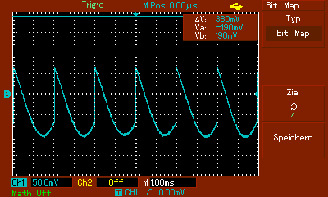
\includegraphics{Lock_In Bilder/Aufgabe 3/MAP004.pdf}
                \caption{AC-Signal bei 135° Phase}
                \label{fig:135sig2}
            \end{figure}
            \\
           
            \begin{figure}
                \centering
                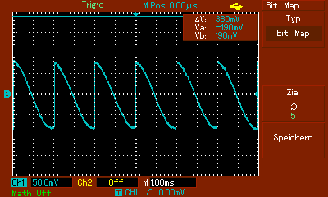
\includegraphics{Lock_In Bilder/Aufgabe 3/MAP005.pdf}
                \caption{AC-Signal bei 180° Phase}
                \label{fig:180sig2}
            \end{figure}
            \\
          
        \item{Experiment mit der Leuchtdiode \\}
        \\
            \begin{figure}
                \centering
                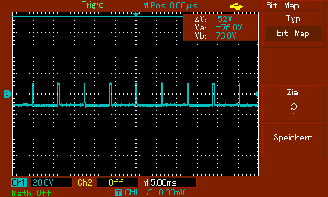
\includegraphics{Lock_In Bilder/Aufgabe 4/MAP001.pdf}
                \caption{Signal bei 5cm}
                \label{fig:5cmled}
            \end{figure}  
            \\
            \begin{figure}   
                \centering 
                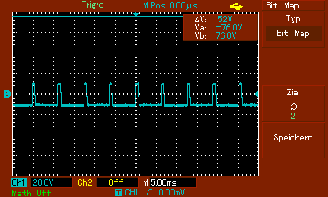
\includegraphics{Lock_In Bilder/Aufgabe 4/MAP002.pdf}
                \caption{Signal bei 10cm}
                \label{fig:10cmled}
            \end{figure}   
            \\
            \begin{figure}    
                \centering
                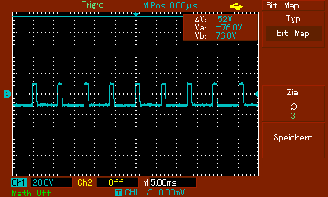
\includegraphics{Lock_In Bilder/Aufgabe 4/MAP003.pdf}
                \caption{Signal bei 15cm}
                \label{fig:15cmled}
            \end{figure}   
            \\
            \begin{figure} 
                \centering  
                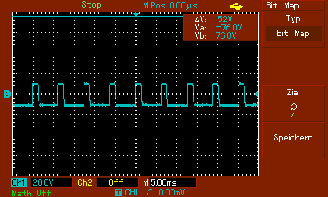
\includegraphics{Lock_In Bilder/Aufgabe 4/MAP004.pdf}
                \caption{Signal bei 20cm}
                \label{fig:20cmled}    
            \end{figure}
            \\
        Die sich vergrößernden Abstände in den Signalen in Mikrosekunden zeigen die Abschwächung des Lichtsignals.
            \begin{figure}
                \centering
                \includegraphics[scale=0.75]{build/graph.pdf}
                \caption{Messwerte des LED-Abstands}
                \label{fig:graph}
            \end{figure}
        \\
        Der Graph ist eine Veranschaulichung der Messwerte und ihre Korrelation zu einem \(1/r²\) Abstand.
    \end{itemize}
\section{Diskussion}
Der Unterschied zwischen den Messungen im ersten Experiment resultiert aus der Tatsache, dass der Tiefpass die Eingangsspannung integriert und mittelt. Von daher entsteht ein Gleichstrom statt eine Schwingung.
Die durch den Bandpass erzwungene Sägezahnkurve entsteht aus der Überlagerung von \(U_{ref}\) und \(U_{sig}\).
In den Bildern des zweiten und dritten Experiments scheint die Kurve sich zu spiegeln. Dies entspricht den Erwartungen, da der Phasenunterschied zwischen \(U_{ref}\) und \(U_{sig}\) sich um genau 180 Grad verschiebt und nach Gleichung (5) ändert sich auch das Vorzeichen von der Gesamtspannung.
Im letzten Experiment wurden vier Messungen aufgenommen.
Die Kurve weist eine \(r²\)-Abhängigkeit auf, weil der durch den Lock-In Verstärker hervorgerufenen Gap in Mikrosekunden als X-Achse gewählt wurde. Diese Gaps werden länger je größer die Distanz zwischen Sender und Empfänger ist. Die Intensität des Lichts weist eine \(1/r²\)-Abhängigkeit auf, wobei sie eben eine Antiproportionalität zu dem, also eine \(r²\)-Abhängigkeit aufweisen.
\newpage
 %Die Hyperlinks funktioneren plötzlich nicht.
\end{document}